\documentclass[11pt, aspectratio=169]{beamer}

% LuaLaTeXで日本語を使うための必須パッケージ
\usepackage{luatexja}

% 便利な追加パッケージ
\usepackage{tikz}
\usetikzlibrary{positioning, calc, shapes.geometric} % shapes.geometric を追加
\usepackage{booktabs}   % 表の罫線
\usepackage{tikz}       % 図形描画
\usepackage{listings}   % ソースコード挿入
\lstset{
  basicstyle=\ttfamily\scriptsize,
  frame=single,
  breaklines=true,
  numbers=left,
  numberstyle=\tiny
}

% テーマとカラーテーマの設定
\usetheme{Madrid}
\usecolortheme{orchid}

% セクション開始時の自動表紙（扉絵）設定
\AtBeginSection[]{
  \begin{frame}
    \vfill
    \centering
    \begin{beamercolorbox}[sep=8pt,center,shadow=true,rounded=true]{title}
      \usebeamerfont{title}\insertsectionhead\par%
    \end{beamercolorbox}
    \vfill
  \end{frame}
}

% タイトル情報
\title{研究室セミナー第2回}
\subtitle{SAGIN}
\author{学籍番号(Student ID): 1280391 \\ 氏名(Name): 細川夏風(Hosokawa Natsuka)}
\institute{高知工科大学(Kochi Univ of Tech)}
\date{\today}

\begin{document}

% タイトルスライド
\begin{frame}
    \titlepage
\end{frame}

% 目次スライド
\begin{frame}{目次}
    \tableofcontents
\end{frame}

% ==========================================
% ここから本文
% ==========================================

\section{はじめに/Intro}

\begin{frame}{SAGINについて}
  \begin{columns}[c]
    \begin{column}{0.4\textwidth}
      \texttt{SAGIN}とは，宇宙・航空・地上統合ネットワークのことである．衛星システム，航空ネットワーク，地上通信を統合する新しいネットワークアーキテクチャである．

      これにより以下の\texttt{6G}要件を満たすことが期待されている．
      \begin{itemize}
        \item 広域アクセス
        \item 大規模接続
        \item 高精度測位
      \end{itemize}
    \end{column}
    \begin{column}{0.6\textwidth}
      \begin{center}
        % resizeboxで図の横幅をカラムの幅(\linewidth)に合わせる
        \resizebox{\linewidth}{!}{
          \begin{tikzpicture}[
            node distance=2.5cm,
            segment/.style={draw, rounded corners, align=center, minimum width=8cm, minimum height=1.2cm, font=\sffamily\bfseries},
            link/.style={<->, thick, >=stealth}
        ]
            % ノードの定義
            \node[segment, fill=blue!15] (space) {宇宙ネットワーク (Space Network)};
            \node[segment, fill=green!15, below of=space] (air) {航空ネットワーク (Air Network)};
            \node[segment, fill=orange!15, below of=air] (ground) {地上ネットワーク (Ground Network)};

            % 垂直方向のリンク
            \draw[link] (space.south) -- (air.north) node[midway, right] {\small Space-Air};
            \draw[link] (air.south) -- (ground.north) node[midway, right] {\small Air-Ground};

            % 宇宙と地上の直接リンク
            \draw[link] (space.west) to[out=210, in=150] node[midway, left] {\small Space-Ground} (ground.west);
          \end{tikzpicture}
        }
      \end{center}
    \end{column}
  \end{columns}
\end{frame}

\begin{frame}{About SAGIN}
  \begin{columns}[c]
    \begin{column}{0.4\textwidth}
      \texttt{SAGIN} stands for Space-Air-Ground Integrated Network. It is a novel network architecture that integrates satellite systems, air networks, and terrestrial communications.

      It is expected to meet various \texttt{6G} requirements, including:
      \begin{itemize}
        \item Wide-area broadband access
        \item Large-scale connectivity
        \item High-precision positioning
      \end{itemize}
    \end{column}
    \begin{column}{0.6\textwidth}
      \begin{center}
        % Use resizebox to scale the TikZ diagram to column width
        \resizebox{\linewidth}{!}{
          \begin{tikzpicture}[
            node distance=2.5cm,
            segment/.style={draw, rounded corners, align=center, minimum width=8cm, minimum height=1.2cm, font=\sffamily\bfseries},
            link/.style={<->, thick, >=stealth}
        ]
            % Definition of nodes
            \node[segment, fill=blue!15] (space) {Space Network};
            \node[segment, fill=green!15, below of=space] (air) {Air Network};
            \node[segment, fill=orange!15, below of=air] {Ground Network};

            % Vertical links
            \draw[link] (space.south) -- (air.north) node[midway, right] {\small Space-Air};
            \draw[link] (air.south) -- (ground.north) node[midway, right] {\small Air-Ground};

            % Direct link between Space and Ground
            \draw[link] (space.west) to[out=210, in=150] node[midway, left] {\small Space-Ground} (ground.west);
          \end{tikzpicture}
        }
      \end{center}
    \end{column}
  \end{columns}
\end{frame}

\begin{frame}{なぜSAGINが必要なのか/Why we need SAGIN}
  より広域により低遅延で通信を実現しようとした場合，現行の通信方式ではアクセスの柔軟性も低いうえに遅延が大きいという課題がある．

  そのため，\texttt{SAGIN}を導入し，シームレスに様々な領域を超えた統合ネットワークを構築する必要がある．

  \vspace{1cm}

  When aiming for communication with wider coverage and lower latency, current communication systems face the challenges of poor access flexibility and high latency.

  Therefore, it is necessary to introduce \texttt{SAGIN} and build an integrated network that seamlessly transcends various domains.
\end{frame}

\section{アーキテクチャ/Architecture}

\begin{frame}{宇宙ネットワーク}
  \begin{columns}[c]
    \begin{column}{0.5\textwidth}
      このネットワークは異なる軌道にある衛星と地上の基地局，ネットワークオペレータ，制御センターなどの対応する地上のインフラ施設や設備で構成されている．衛星は高度に応じて，静止衛星(\texttt{GEO})，中軌道衛星(\texttt{MEO})，低軌道衛星(\texttt{LEO})の$3$つのカテゴリに分類されている．

      \vspace{1em}

      これらの衛星同士が多層衛星ネットワーク(\texttt{MLSN})を構成している．これには衛星間リンク(\texttt{ISL})や層間リンク(\texttt{ILL})などの複数リンクタイプが存在する．
    \end{column}
    \begin{column}{0.5\textwidth}
      \begin{center}
        % 0.65 * 1.07 = 約0.70 に拡大
        \resizebox{!}{0.70\textheight}{
        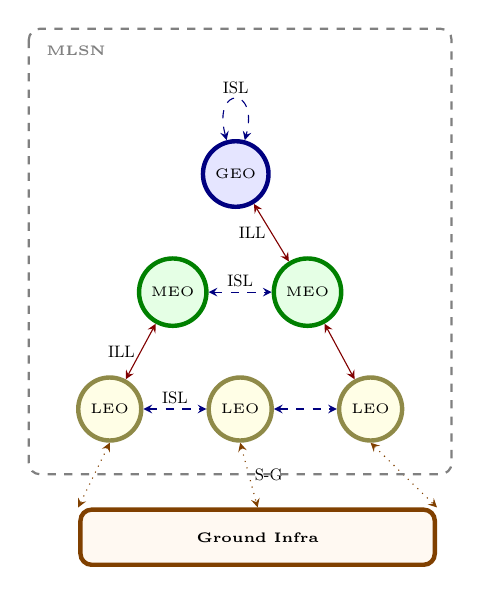
\begin{tikzpicture}[
            node distance=0.5cm and 0.8cm,
            sat/.style={circle, draw, minimum size=0.6cm, align=center, font=\tiny, ultra thick},
            geo/.style={sat, fill=blue!10, draw=blue!50!black},
            meo/.style={sat, fill=green!10, draw=green!50!black},
            leo/.style={sat, fill=yellow!10, draw=yellow!50!black},
            ground/.style={rectangle, draw, rounded corners, fill=orange!5, minimum width=4.5cm, minimum height=0.7cm, align=center, font=\tiny\bfseries, ultra thick, draw=orange!50!black},
            link/.style={<->, thin, >=stealth},
            isl/.style={link, blue!50!black, dashed},
            ill/.style={link, red!50!black},
            glink/.style={link, orange!50!black, dotted}
        ]
            % --- ノード配置 ---
            \node[ground] (infra) {Ground Infra};
            \node[leo, above=1.2cm of infra.west, xshift=0.4cm] (leo1) {LEO};
            \node[leo, right=of leo1] (leo2) {LEO};
            \node[leo, right=of leo2] (leo3) {LEO};
            \node[meo, above=0.6cm of leo1, xshift=0.8cm] (meo1) {MEO};
            \node[meo, right=of meo1] (meo2) {MEO};
            \node[geo, above=0.6cm of meo1, xshift=0.8cm] (geo1) {GEO};

            % --- リンク描画 ---
            \draw[isl] (geo1) to[loop above] node[above, black, scale=0.6] {ISL} (geo1); 
            \draw[isl] (meo1) -- node[above, black, scale=0.6] {ISL} (meo2);
            \draw[isl] (leo1) -- node[above, black, scale=0.6] {ISL} (leo2);
            \draw[isl] (leo2) -- (leo3);
            
            \draw[ill] (geo1) -- node[midway, left, black, scale=0.6] {ILL} (meo2);
            \draw[ill] (meo1) -- node[midway, left, black, scale=0.6] {ILL} (leo1);
            \draw[ill] (meo2) -- (leo3);
            
            \draw[glink] (leo1.south) -- (infra.north west);
            \draw[glink] (leo2.south) -- node[midway, right, black, scale=0.6] {S-G} (infra.north);
            \draw[glink] (leo3.south) -- (infra.north east);

            % --- MLSN枠の修正（バランス調整） ---
            % 左端をleo1、右端をleo3、上端をgeo1(のISL分)を基準にして左右対称に
            \draw[dashed, gray, thick, rounded corners] 
              ($(leo1.west |- geo1.north)+(-0.6cm,1.4cm)$) rectangle ($(leo3.east |- leo3.south)+(0.6cm,-0.4cm)$);
            
            \node[anchor=north west, font=\tiny\bfseries, gray] 
              at ($(leo1.west |- geo1.north)+(-0.5cm,1.3cm)$) {MLSN};

        \end{tikzpicture}
        }
      \end{center}
    \end{column}
  \end{columns}
\end{frame}

\subsection{宇宙ネットワーク/Space Network}

\begin{frame}{Space Network}
  \begin{columns}[c]
    \begin{column}{0.5\textwidth}
      \small % 英語は文字数が多くなりやすいため、少しだけ小さくすると収まりが良いです
      This network consists of satellites in various orbits and corresponding ground infrastructure facilities and equipment, such as base stations, network operators, and control centers.

      \vspace{1em}
      Satellites are classified into three categories based on altitude: Geostationary Earth Orbit (\texttt{GEO}), Medium Earth Orbit (\texttt{MEO}), and Low Earth Orbit (\texttt{LEO}).

      \vspace{1em}
      These satellites form a Multi-Layer Satellite Network (\texttt{MLSN}), which utilizes multiple link types such as Inter-Satellite Links (\texttt{ISL}) and Inter-Layer Links (\texttt{ILL}).
    \end{column}
    \begin{column}{0.5\textwidth}
      \begin{center}
        \resizebox{!}{0.70\textheight}{
        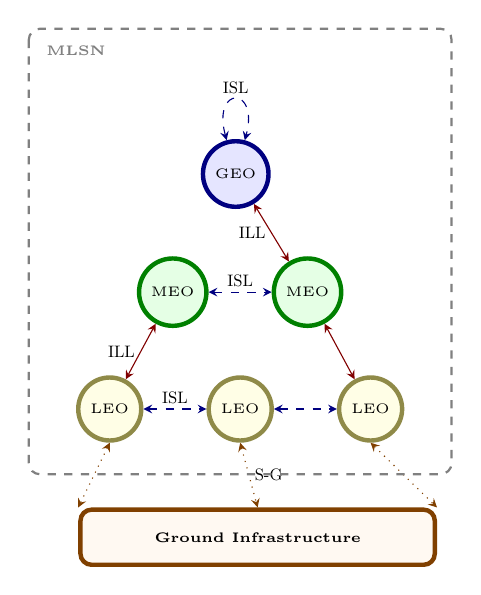
\begin{tikzpicture}[
            node distance=0.5cm and 0.8cm,
            sat/.style={circle, draw, minimum size=0.6cm, align=center, font=\tiny, ultra thick},
            geo/.style={sat, fill=blue!10, draw=blue!50!black},
            meo/.style={sat, fill=green!10, draw=green!50!black},
            leo/.style={sat, fill=yellow!10, draw=yellow!50!black},
            ground/.style={rectangle, draw, rounded corners, fill=orange!5, minimum width=4.5cm, minimum height=0.7cm, align=center, font=\tiny\bfseries, ultra thick, draw=orange!50!black},
            link/.style={<->, thin, >=stealth},
            isl/.style={link, blue!50!black, dashed},
            ill/.style={link, red!50!black},
            glink/.style={link, orange!50!black, dotted}
        ]
            % --- Node Placement ---
            \node[ground] (infra) {Ground Infrastructure};
            \node[leo, above=1.2cm of infra.west, xshift=0.4cm] (leo1) {LEO};
            \node[leo, right=of leo1] (leo2) {LEO};
            \node[leo, right=of leo2] (leo3) {LEO};
            \node[meo, above=0.6cm of leo1, xshift=0.8cm] (meo1) {MEO};
            \node[meo, right=of meo1] (meo2) {MEO};
            \node[geo, above=0.6cm of meo1, xshift=0.8cm] (geo1) {GEO};

            % --- Link Drawing ---
            \draw[isl] (geo1) to[loop above] node[above, black, scale=0.6] {ISL} (geo1);
            \draw[isl] (meo1) -- node[above, black, scale=0.6] {ISL} (meo2);
            \draw[isl] (leo1) -- node[above, black, scale=0.6] {ISL} (leo2);
            \draw[isl] (leo2) -- (leo3);

            \draw[ill] (geo1) -- node[midway, left, black, scale=0.6] {ILL} (meo2);
            \draw[ill] (meo1) -- node[midway, left, black, scale=0.6] {ILL} (leo1);
            \draw[ill] (meo2) -- (leo3);

            \draw[glink] (leo1.south) -- (infra.north west);
            \draw[glink] (leo2.south) -- node[midway, right, black, scale=0.6] {S-G} (infra.north);
            \draw[glink] (leo3.south) -- (infra.north east);

            % --- MLSN Box Correction ---
            \draw[dashed, gray, thick, rounded corners]
              ($(leo1.west |- geo1.north)+(-0.6cm,1.4cm)$) rectangle ($(leo3.east |- leo3.south)+(0.6cm,-0.4cm)$);

            \node[anchor=north west, font=\tiny\bfseries, gray]
              at ($(leo1.west |- geo1.north)+(-0.5cm,1.3cm)$) {MLSN};

        \end{tikzpicture}
        }
      \end{center}
    \end{column}
  \end{columns}
\end{frame}

\begin{frame}[c]{静止衛星 (GEO) / Geostationary Earth Orbit}
  \begin{columns}[c]
    \begin{column}{0.45\textwidth}
      地上に対して固定された高軌道の位置に存在する．単一の衛星で地球の面積の 42\% をカバー可能．3 ～ 4 機で極地を含みカバー可能．ただ，一方向の遅延が大きく約 270ms 程となっている．

      \vspace{1em}
      \textit{GEO satellites are located in a fixed high-altitude orbit relative to the ground. A single satellite can cover 42\% of the Earth's area, and 3--4 satellites can provide coverage including the polar regions. However, the one-way delay is large, at approximately 270ms.}
    \end{column}

    \begin{column}{0.5\textwidth}
      \begin{center}
        \resizebox{!}{0.65\textheight}{
        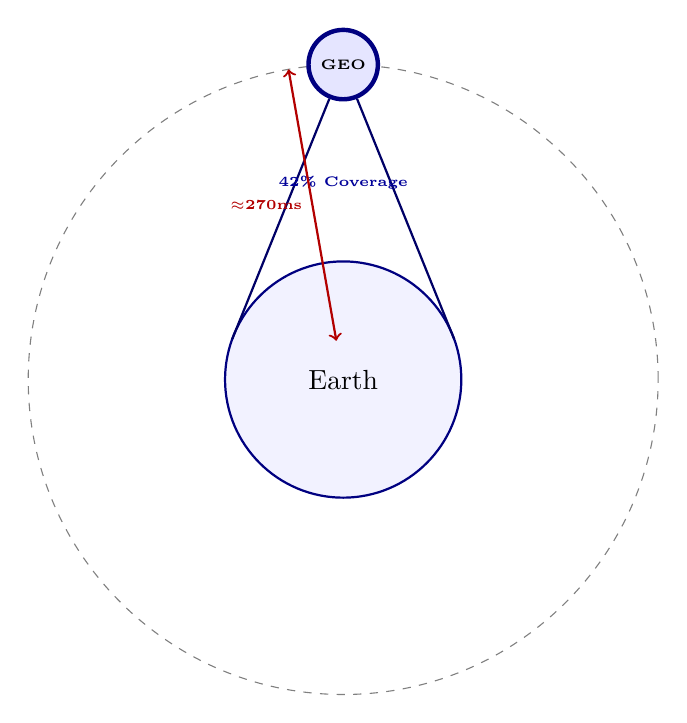
\begin{tikzpicture}[sat/.style={circle, fill=blue!10, draw=blue!50!black, ultra thick, minimum size=0.8cm, font=\tiny\bfseries}]
            \draw[fill=blue!5, draw=blue!50!black, thick] (0,0) circle (1.5);
            \node at (0,0) {Earth};
            \draw[dashed, gray] (0,0) circle (4);
            \node[sat] (s) at (90:4) {GEO};
            \draw[blue!40!black, thick] (s) -- (160:1.5);
            \draw[blue!40!black, thick] (s) -- (20:1.5);
            \node[blue!60!black, font=\tiny\bfseries] at (90:2.5) {42\% Coverage};
            \draw[<->, red!70!black, thick] (100:0.5) -- (100:4) node[midway, left, font=\tiny\bfseries] {$\approx$270ms};
        \end{tikzpicture}
        }
      \end{center}
    \end{column}
  \end{columns}
\end{frame}

\begin{frame}[c]{中軌道衛星 (MEO) / Medium Earth Orbit}
  \begin{columns}[c]
    \begin{column}{0.5\textwidth}
      \small
      高度が 2000km ～ 20000km の位置し，地球面積の 12\% ～ 38\% 程をカバーし，10 機以上で全体をカバー可能．高帯域幅，低コスト低遅延を実現可能に設定されている．システムの容量が最大 15Gbps になる．文献 \cite{chen2023sagin} では，遅延は 110ms とされている．

      \vspace{1em}
      \textit{Located at altitudes of 2,000km to 20,000km, MEO satellites cover about 12\% to 38\% of the Earth's area and can cover the entire globe with 10 or more satellites. They are designed to achieve high bandwidth, low cost, and low latency. The system capacity reaches up to 15Gbps. In literature \cite{chen2023sagin}, the latency is stated as 110ms.}
    \end{column}

    \begin{column}{0.5\textwidth}
      \begin{center}
        \resizebox{!}{0.65\textheight}{
        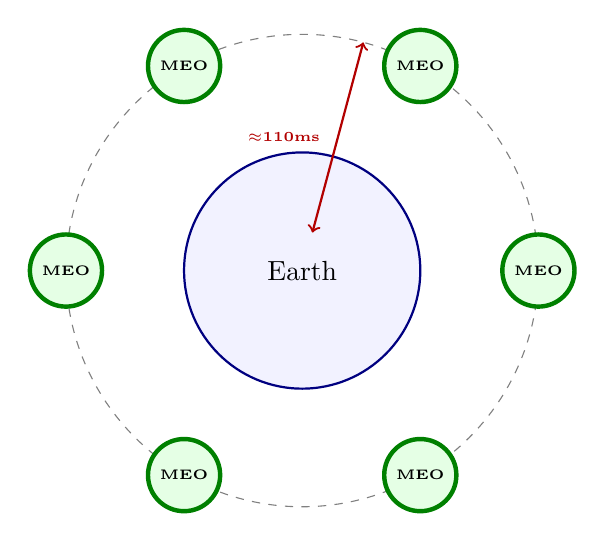
\begin{tikzpicture}[sat/.style={circle, fill=green!10, draw=green!50!black, ultra thick, minimum size=0.6cm, font=\tiny\bfseries}]
            \draw[fill=blue!5, draw=blue!50!black, thick] (0,0) circle (1.5);
            \node at (0,0) {Earth};
            \draw[dashed, gray] (0,0) circle (3);
            \foreach \a in {0, 60, 120, 180, 240, 300} {
                \node[sat] at (\a:3) {MEO};
            }
            \draw[<->, red!70!black, thick] (75:0.5) -- (75:3) node[midway, left, font=\tiny\bfseries, xshift=-0.1cm] {$\approx$110ms};
        \end{tikzpicture}
        }
      \end{center}
    \end{column}
  \end{columns}
\end{frame}

\begin{frame}[c]{低軌道衛星 (LEO) / Low Earth Orbit}
  \begin{columns}[c]
    \begin{column}{0.45\textwidth}
      低コストで構築可能だが，グローバル通信を実現するためには多数の衛星が必要．伝播距離が短いため，遅延が 40ms 未満と小さい．地上に対して移動速度が大きいため，通信を安定させることが難しい．

      \vspace{1em}
      \textit{LEO satellites can be built at low cost but require a large number of satellites to achieve global communication. Due to the short propagation distance, the delay is small, less than 40ms. Since the movement speed relative to the ground is high, it is difficult to stabilize communication.}
    \end{column}

    \begin{column}{0.5\textwidth}
      \begin{center}
        \resizebox{!}{0.65\textheight}{
        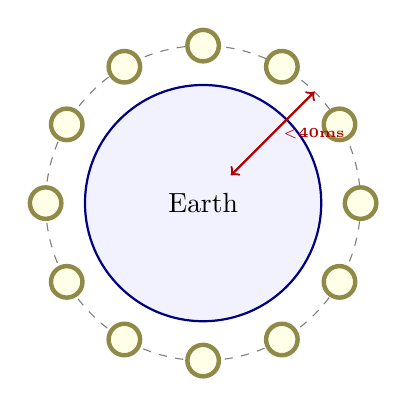
\begin{tikzpicture}[sat/.style={circle, fill=yellow!10, draw=yellow!50!black, ultra thick, minimum size=0.4cm, font=\tiny\bfseries}]
            \draw[fill=blue!5, draw=blue!50!black, thick] (0,0) circle (1.5);
            \node at (0,0) {Earth};
            \draw[dashed, gray] (0,0) circle (2);
            \foreach \a in {0, 30, 60, 90, 120, 150, 180, 210, 240, 270, 300, 330} {
                \node[sat] at (\a:2) {};
            }
            \draw[<->, red!70!black, thick] (45:0.5) -- (45:2) node[midway, right, font=\tiny\bfseries] {$<$40ms};
        \end{tikzpicture}
        }
      \end{center}
    \end{column}
  \end{columns}
\end{frame}

\subsection{航空ネットワーク/Air Network}

\begin{frame}[c]{航空ネットワーク}
  \begin{columns}[c]
    \begin{column}{0.5\textwidth}
      このネットワークは航空機器（航空機，気球，\texttt{UAV}：無人航空機）をキャリアとして使用し，情報の送信、処理を行うモバイルシステムである．
      
      \vspace{0.5em}
      宇宙ネットワークと同様に高度によって，高高度プラットフォーム (\texttt{HAPs})，低高度プラットフォーム (\texttt{LAPs}) に分類できる．
      
      \vspace{0.5em}
      地上基地局と比較して展開が容易でカバー範囲が広く，地域のワイヤレスアクセスを提供可能である．また，構築コストは宇宙ネットワークの運用よりも遥かに低く抑えられる．
    \end{column}

    \begin{column}{0.48\textwidth}
      \begin{center}
        \resizebox{!}{0.65\textheight}{
        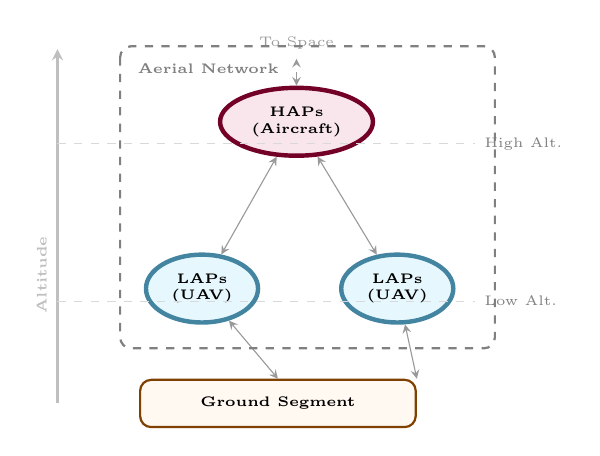
\begin{tikzpicture}[
            node distance=0.6cm and 1.0cm,
            ground/.style={rectangle, draw, rounded corners, fill=orange!5, minimum width=3.5cm, minimum height=0.6cm, align=center, font=\tiny\bfseries, thick, draw=orange!50!black},
            platform/.style={ellipse, draw, ultra thick, minimum width=1.2cm, minimum height=0.7cm, align=center, font=\tiny\bfseries},
            haps/.style={platform, fill=purple!10, draw=purple!60!black},
            laps/.style={platform, fill=cyan!10, draw=cyan!60!black},
            link/.style={<->, thin, >=stealth, gray!80},
            axis/.style={->, thick, >=stealth, gray!50}
        ]
            % --- 1. ノード配置（xshiftを増やして軸から離す） ---
            \node[ground] (infra) at (1,0) {Ground Segment};
            
            \node[laps, above=1.0cm of infra.west, xshift=0.8cm] (lap1) {LAPs\\(UAV)};
            \node[laps, right=of lap1] (lap2) {LAPs\\(UAV)};
            
            \node[haps, above=1.2cm of lap1, xshift=1.2cm] (hap1) {HAPs\\(Aircraft)};

            % --- 2. リンク ---
            \draw[link] (hap1) -- (lap1);
            \draw[link] (hap1) -- (lap2);
            \draw[link] (lap1) -- (infra.north);
            \draw[link] (lap2) -- (infra.north east);
            \draw[link, dashed] (hap1) -- ++(0,0.8) node[above, font=\tiny] {To Space};

            % --- 3. 高度軸（位置を左にオフセット） ---
            \draw[axis] (-1.8,0) -- (-1.8,4.5) node[midway, left, rotate=90, font=\tiny\bfseries, yshift=0.2cm] {Altitude};
            \draw[dashed, gray!30] (-1.8,1.3) -- (3.5,1.3) node[right, font=\tiny, gray] {Low Alt.};
            \draw[dashed, gray!30] (-1.8,3.3) -- (3.5,3.3) node[right, font=\tiny, gray] {High Alt.};

            % --- 4. 範囲（枠も重ならないように調整） ---
            \draw[dashed, gray, thick, rounded corners] 
              ($(lap1.west |- hap1.north)+(-0.3cm,0.5cm)$) rectangle ($(lap2.east |- lap1.south)+(0.5cm,-0.3cm)$);
            \node[anchor=north west, font=\tiny\bfseries, gray] 
              at ($(lap1.west |- hap1.north)+(-0.2cm,0.4cm)$) {Aerial Network};

        \end{tikzpicture}
        }
      \end{center}
    \end{column}
  \end{columns}
\end{frame}

\begin{frame}[c]{Aerial Network}
  \begin{columns}[c]
    \begin{column}{0.5\textwidth}
      This network is a mobile system that uses aerial equipment (aircraft, balloons, and, \texttt{UAVs}: Unmanned Aerial Vehicles) as carriers to transmit and process information.

      \vspace{0.5em}
      Similar to space networks, it can be classified into High Altitude Platforms (\texttt{HAPs}) and Low Altitude Platforms (\texttt{LAPs}) based on altitude.

      \vspace{0.5em}
      Compared to ground network base stations, aerial networks are easier to deploy and offer wider coverage. They can provide regional wireless access. At the same time, the deployment cost is significantly lower than that of operating a space network.
    \end{column}

    \begin{column}{0.48\textwidth}
      \begin{center}
        \resizebox{!}{0.65\textheight}{
        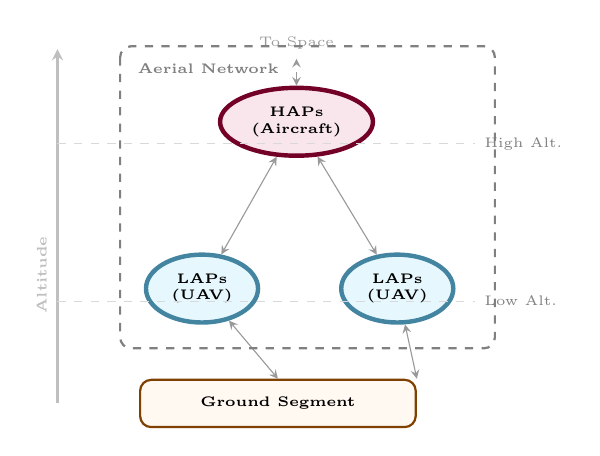
\begin{tikzpicture}[
            node distance=0.6cm and 1.0cm,
            ground/.style={rectangle, draw, rounded corners, fill=orange!5, minimum width=3.5cm, minimum height=0.6cm, align=center, font=\tiny\bfseries, thick, draw=orange!50!black},
            platform/.style={ellipse, draw, ultra thick, minimum width=1.2cm, minimum height=0.7cm, align=center, font=\tiny\bfseries},
            haps/.style={platform, fill=purple!10, draw=purple!60!black},
            laps/.style={platform, fill=cyan!10, draw=cyan!60!black},
            link/.style={<->, thin, >=stealth, gray!80},
            axis/.style={->, thick, >=stealth, gray!50}
        ]
            % --- Node Placement ---
            \node[ground] (infra) at (1,0) {Ground Segment};
            \node[laps, above=1.0cm of infra.west, xshift=0.8cm] (lap1) {LAPs\\(UAV)};
            \node[laps, right=of lap1] (lap2) {LAPs\\(UAV)};
            \node[haps, above=1.2cm of lap1, xshift=1.2cm] (hap1) {HAPs\\(Aircraft)};

            % --- Links ---
            \draw[link] (hap1) -- (lap1);
            \draw[link] (hap1) -- (lap2);
            \draw[link] (lap1) -- (infra.north);
            \draw[link] (lap2) -- (infra.north east);
            \draw[link, dashed] (hap1) -- ++(0,0.8) node[above, font=\tiny] {To Space};

            % --- Altitude Axis (Offset to the left) ---
            \draw[axis] (-1.8,0) -- (-1.8,4.5) node[midway, left, rotate=90, font=\tiny\bfseries, yshift=0.2cm] {Altitude};
            \draw[dashed, gray!30] (-1.8,1.3) -- (3.5,1.3) node[right, font=\tiny, gray] {Low Alt.};
            \draw[dashed, gray!30] (-1.8,3.3) -- (3.5,3.3) node[right, font=\tiny, gray] {High Alt.};

            % --- Box ---
            \draw[dashed, gray, thick, rounded corners]
              ($(lap1.west |- hap1.north)+(-0.3cm,0.5cm)$) rectangle ($(lap2.east |- lap1.south)+(0.5cm,-0.3cm)$);
            \node[anchor=north west, font=\tiny\bfseries, gray]
              at ($(lap1.west |- hap1.north)+(-0.2cm,0.4cm)$) {Aerial Network};

        \end{tikzpicture}
        }
      \end{center}
    \end{column}
  \end{columns}
\end{frame}

\begin{frame}[c]{高高度・低高度プラットフォーム}
  \begin{columns}[c]
    \begin{column}{0.5\textwidth}
      \small
      \begin{itemize}
        \item \texttt{HAPs} の役割

        衛星との接続にも用いられ，分散型のデータセンターとして機能している．経路の記録やお互いの監視などを行う．これらの情報は衛星と通信を行うために重要である．地上とのワイヤレスでの接続のためのサービスを提供するためにも用いられる．
      \item \texttt{LAPs} の役割

        このプラットフォーム\texttt{UAV}は重要な役割を持っており，\texttt{HAPs}より柔軟性が高い．適切な通信管理を行うことによって通信のオーバヘッドを減少させることができる．\texttt{UAV}は様々な通信の分散処理能力の向上や移動体の基地局としてモバイルのクライドコンピューティングのシステムとしてももいいることができると考えられている．
      \end{itemize}
    \end{column}

    \begin{column}{0.48\textwidth}
      \begin{center}
        \resizebox{!}{0.6\textheight}{
        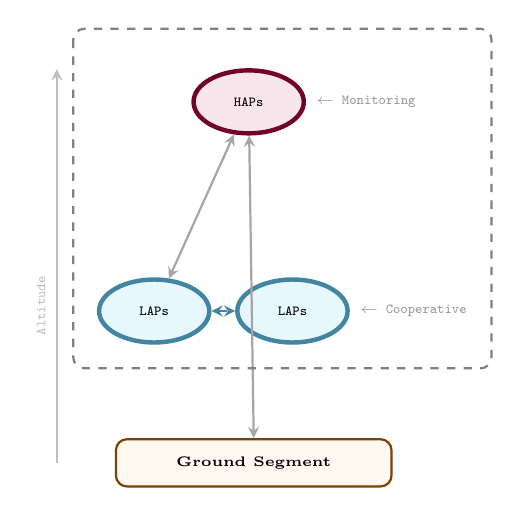
\begin{tikzpicture}[
            node distance=0.8cm and 1.2cm,
            platform/.style={ellipse, draw, ultra thick, minimum width=1.4cm, minimum height=0.8cm, align=center, font=\tiny\ttfamily},
            haps/.style={platform, fill=purple!10, draw=purple!60!black},
            laps/.style={platform, fill=cyan!10, draw=cyan!60!black},
            infra/.style={rectangle, draw, rounded corners, fill=orange!5, minimum width=3.5cm, minimum height=0.6cm, align=center, font=\tiny\bfseries, thick, draw=orange!50!black},
            label/.style={font=\tiny\ttfamily, gray!80},
            link/.style={<->, thick, >=stealth, gray!70},
            axis/.style={->, thick, >=stealth, gray!50}
        ]
            % --- ノード配置 ---
            \node[infra] (ground) at (1.5,0) {Ground Segment};
            \node[laps, above=1.5cm of ground.west, xshift=0.5cm] (lap1) {LAPs};
            \node[laps, right=0.3cm of lap1] (lap2) {LAPs};
            \draw[link, dashed, cyan!60!black] (lap1) -- (lap2);
            \node[haps, above=1.8cm of lap1, xshift=1.2cm] (hap1) {HAPs};

            % --- リンクとラベル ---
            \draw[link] (hap1) -- (lap1);
            \draw[link] (hap1) -- (ground.north);
            \draw[axis] (-1.0,0) -- (-1.0,5.0) node[midway, left, rotate=90, font=\tiny\ttfamily, yshift=0.2cm] {Altitude};
            \node[label, anchor=west] at (hap1.east) {$\leftarrow$ Monitoring};
            \node[label, anchor=west] at (lap2.east) {$\leftarrow$ Cooperative};

            % 範囲枠
            \draw[dashed, gray, thick, rounded corners]
              ($(lap1.west |- hap1.north)+(-0.3cm,0.5cm)$) rectangle ($(lap2.east |- lap1.south)+(1.8cm,-0.3cm)$);
        \end{tikzpicture}
        }
      \end{center}
    \end{column}
  \end{columns}
\end{frame}

\begin{frame}[c]{High and Low Altitude Platforms}
  \begin{columns}[c]
    \begin{column}{0.5\textwidth}
      \scriptsize
      \begin{itemize}
        \item Roles of \texttt{HAPs} \\
        They are used for connections with satellites and function as distributed data centers. They perform tasks such as recording trajectories and mutual monitoring. This information is important for conducting communication with satellites. They are also used to provide services for wireless connections with the ground.

        \vspace{0.5em}
        \item Roles of \texttt{LAPs} \\
        \texttt{UAV}s are mainly used for this platform, offering higher flexibility than \texttt{HAPs}. Communication overhead can be reduced by performing appropriate communication management. \texttt{UAV}s play an important role in this platform; it is considered that they can be used to improve various distributed processing capabilities of communications and serve as mobile base stations for mobile cloud computing systems.
      \end{itemize}
    \end{column}

    \begin{column}{0.48\textwidth}
      \begin{center}
        \resizebox{!}{0.6\textheight}{
        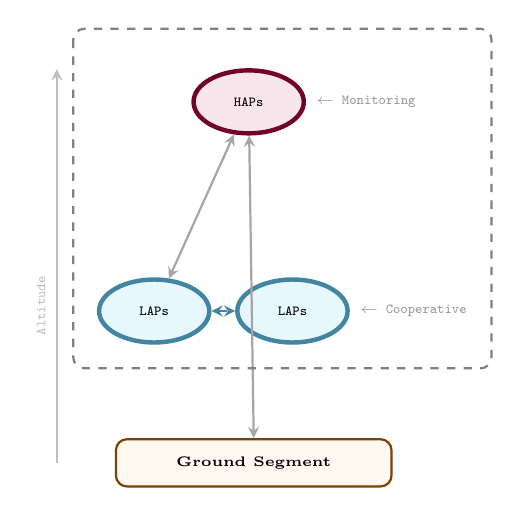
\begin{tikzpicture}[
            node distance=0.8cm and 1.2cm,
            platform/.style={ellipse, draw, ultra thick, minimum width=1.4cm, minimum height=0.8cm, align=center, font=\tiny\ttfamily},
            haps/.style={platform, fill=purple!10, draw=purple!60!black},
            laps/.style={platform, fill=cyan!10, draw=cyan!60!black},
            infra/.style={rectangle, draw, rounded corners, fill=orange!5, minimum width=3.5cm, minimum height=0.6cm, align=center, font=\tiny\bfseries, thick, draw=orange!50!black},
            label/.style={font=\tiny\ttfamily, gray!80},
            link/.style={<->, thick, >=stealth, gray!70},
            axis/.style={->, thick, >=stealth, gray!50}
        ]
            % --- Node Placement ---
            \node[infra] (ground) at (1.5,0) {Ground Segment};
            \node[laps, above=1.5cm of ground.west, xshift=0.5cm] (lap1) {LAPs};
            \node[laps, right=0.3cm of lap1] (lap2) {LAPs};
            \draw[link, dashed, cyan!60!black] (lap1) -- (lap2);
            \node[haps, above=1.8cm of lap1, xshift=1.2cm] (hap1) {HAPs};

            % --- Links and Labels ---
            \draw[link] (hap1) -- (lap1);
            \draw[link] (hap1) -- (ground.north);
            \draw[axis] (-1.0,0) -- (-1.0,5.0) node[midway, left, rotate=90, font=\tiny\ttfamily, yshift=0.2cm] {Altitude};
            \node[label, anchor=west] at (hap1.east) {$\leftarrow$ Monitoring};
            \node[label, anchor=west] at (lap2.east) {$\leftarrow$ Cooperative};

            % Bounding Box
            \draw[dashed, gray, thick, rounded corners]
              ($(lap1.west |- hap1.north)+(-0.3cm,0.5cm)$) rectangle ($(lap2.east |- lap1.south)+(1.8cm,-0.3cm)$);
        \end{tikzpicture}
        }
      \end{center}
    \end{column}
  \end{columns}
\end{frame}

\subsection{地上ネットワーク/Ground Network}

\begin{frame}[c]{地上ネットワーク}
  \begin{columns}[c]
    \begin{column}{0.6\textwidth}
      % 標準サイズ（指定なし）
      地上ネットワークは様々なネットワークで構成されている．これらのネットワークは基地局やアクセスポイントを通じてユーザに広範囲かつ低遅延な通信を実現している．
      
      \vspace{0.5em}
      このネットワークは \texttt{SAGIN} の基盤であり，多くの計算資源と高い通信容量を提供できるという特徴がある．
      
      \vspace{0.5em}
      しかし，いくつかの制限も存在している．地形問題や経済問題からカバーしている範囲は地球のわずか数\%にすぎない．また，災害によるリスクも大きい．
    \end{column}

    \begin{column}{0.35\textwidth}
      \begin{center}
        % 幅を0.7倍に縮小
        \resizebox{0.7\linewidth}{!}{
        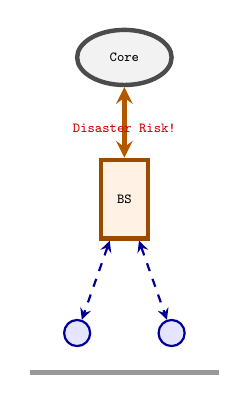
\begin{tikzpicture}[
            bs/.style={rectangle, fill=orange!10, draw=orange!60!black, ultra thick, minimum width=0.6cm, minimum height=1cm, align=center, font=\tiny\ttfamily},
            cloud/.style={draw, ellipse, fill=gray!10, draw=gray!60!black, ultra thick, minimum width=1.2cm, minimum height=0.7cm, font=\tiny\ttfamily},
            user/.style={circle, fill=blue!10, draw=blue!60!black, thick, minimum size=0.3cm},
            link/.style={<->, thick, >=stealth, gray!70},
            fiber/.style={link, ultra thick, orange!70!black},
            wireless/.style={link, dashed, blue!60!black}
        ]
            \node[cloud] (core) at (0,4) {Core};
            \node[bs] (bs) at (0,2.2) {BS};
            \node[user] (u1) at (-0.6,0.5) {};
            \node[user] (u2) at (0.6,0.5) {};

            \draw[fiber] (core) -- (bs);
            \draw[wireless] (bs) -- (u1);
            \draw[wireless] (bs) -- (u2);

            \draw[ultra thick, gray!80] (-1.2,0) -- (1.2,0);
            \node[red!80!black, font=\tiny\ttfamily] at (0,3.1) {Disaster Risk!};
        \end{tikzpicture}
        }
      \end{center}
    \end{column}
  \end{columns}
\end{frame}

\begin{frame}[c]{Ground Network}
  \begin{columns}[c]
    \begin{column}{0.6\textwidth}
      Ground networks consist of various networks. These networks realize wide-range and low-latency communication for users through base stations and access points.
      
      \vspace{0.5em}
      This network is the foundation of \texttt{SAGIN} and is characterized by its ability to provide abundant computational resources and high communication capacity.
      
      \vspace{0.5em}
      However, several limitations also exist. Coverage is limited to a few percent of the Earth due to geographical and economic issues. Furthermore, the risk from disasters is significant.
    \end{column}

    \begin{column}{0.35\textwidth}
      \begin{center}
        % 幅を0.7倍に縮小
        \resizebox{0.7\linewidth}{!}{
        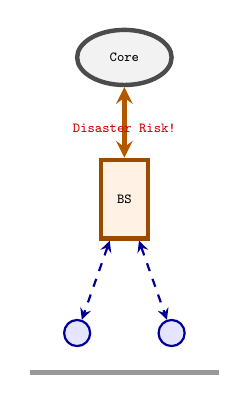
\begin{tikzpicture}[
            bs/.style={rectangle, fill=orange!10, draw=orange!60!black, ultra thick, minimum width=0.6cm, minimum height=1cm, align=center, font=\tiny\ttfamily},
            cloud/.style={draw, ellipse, fill=gray!10, draw=gray!60!black, ultra thick, minimum width=1.2cm, minimum height=0.7cm, font=\tiny\ttfamily},
            user/.style={circle, fill=blue!10, draw=blue!60!black, thick, minimum size=0.3cm},
            link/.style={<->, thick, >=stealth, gray!70},
            fiber/.style={link, ultra thick, orange!70!black},
            wireless/.style={link, dashed, blue!60!black}
        ]
            \node[cloud] (core) at (0,4) {Core};
            \node[bs] (bs) at (0,2.2) {BS};
            \node[user] (u1) at (-0.6,0.5) {};
            \node[user] (u2) at (0.6,0.5) {};

            \draw[fiber] (core) -- (bs);
            \draw[wireless] (bs) -- (u1);
            \draw[wireless] (bs) -- (u2);

            \draw[ultra thick, gray!80] (-1.2,0) -- (1.2,0);
            \node[red!80!black, font=\tiny\ttfamily] at (0,3.1) {Disaster Risk!};
        \end{tikzpicture}
        }
      \end{center}
    \end{column}
  \end{columns}
\end{frame}

\section{}

\end{document}
